\documentclass[12pt,a4paper]{article}

% Paquetes de configuración del documento
\usepackage[utf8]{inputenc}
\usepackage[spanish]{babel}
\usepackage[T1]{fontenc}
\usepackage[margin=2.5cm]{geometry}
\usepackage{fancyhdr}
\usepackage{tabularx}
\usepackage{booktabs}
%Paquetes para simbologia%
\usepackage{amsmath}
\usepackage{amsfonts}
\usepackage{amssymb}
\usepackage{physics}
\usepackage{longtable}
\usepackage{graphicx}
\usepackage{caption}
\usepackage{float}
\usepackage[hyphens]{url}        % Permite cortar URLs largas con guiones
\usepackage[colorlinks=true,
            linkcolor=black,
            urlcolor=myblue,
            citecolor=black,
            filecolor=black]{hyperref}
 % Opción estándar para enlaces
\Urlmuskip=0mu plus 1mu          % Mejora el espaciado para permitir cortes
\usepackage{subcaption}  % en el preámbulo
\usepackage{pgfplots}
\pgfplotsset{compat=1.18}
\usepackage{tikz}
\usepackage{xcolor}
\definecolor{myblue}{RGB}{42, 127, 179}

% Encabezado
\pagestyle{fancy}
\lhead{\textit{Ingeniería Mecánica}}
\chead{\textit{Materiales Metálicos}}
\rhead{\textit{UTN-FRVM}}

\begin{document}
\begin{titlepage}
	
	\begin{center}
		{\huge \textit{Universidad Tecnológica Nacional}}\\
        \vspace{0.5cm}
		{\LARGE \textit{Facultad Regional Villa María}}\\
		\vspace{1.5cm}
        {\LARGE{\textit{Ingeniería Mecánica - Materiales Metálicos}}}\\
		\vspace{1.5cm}
        \LARGE{\textit{Trabajo Práctico 3-06}}
	\end{center}
	
	\vfill

    \textit{Grupo DEL RÍO:}
	\begin{itemize}
		\item \textit{Abregú, Iván.}
		\item \textit{Antico, Rodrigo.}
		\item \textit{Brussa,Julián.}
		\item \textit{Cabral, Franco.}
        \item \textit{Cárdenas, Felipe.}
        \item \textit{Cardozo, Martín.}
        \item \textit{Córdoba, Nathan.}
        \item \textit{Cucco, Ramiro.}
        \item \textit{del Río, Juan.}
        \item \textit{Guerini, Nazareno.}
        \item \textit{Medina, Ivo.}
        \item \textit{Ortiz, Gastón.}
        \item \textit{Picos, Elías.}
        \item \textit{Quinteros, Lautaro.}
	\end{itemize}
    
	\textit{Docentes:}
	\begin{itemize}
		\item \textit{Dr. Lucioni, Eldo José.}
		\item \textit{Ing. Victorio Vallaro, Juan Manuel.}
	\end{itemize}
	\centering
	\today
	
\end{titlepage}

\newpage
\tableofcontents

\begin{abstract}
    A partir de la bibliografía listada a continuación, analice e investigue el contenido relacionado con el ensayo de chispas en acero (Cap. XX) a fin de adquirir efectuar una demostración práctica de sus conocimientos.
    \begin{itemize}
        \item Apraiz Barreiro, J. Aceros Especiales y Otras Aleaciones. Dossat. 5ta Edición. Madrid, 1975. Cap. XX Ensayo de Chispas (pp. 509-520) \{MM-CAD-0.0.0\}
    \end{itemize}
\end{abstract}

\section{Propósito y Fundamento del Ensayo.}

El ensayo de chispa es un método de clasificación de aceros por su composición que se realiza de forma sencilla y económica. Es decir, este método se hace por medio de comparaciones con aceros con composición ya sabida. No se utiliza para un análisis químico detallado, sino como una herramienta complementaria y de control para diferenciar y separar materiales en talleres y almacenes.

\begin{figure}[h]
    \centering
    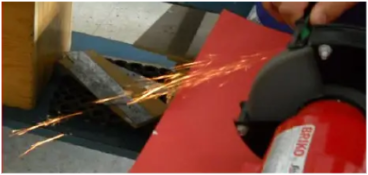
\includegraphics[width=0.7\linewidth]{Figuras/Chispa.png}
    \caption{Ensayo de Chispa.}
    \label{fig:chispa}
\end{figure}

El fundamento del ensayo es la observación de las chispas que se generan al frotar el acero (o como veremos más adelante también con fundiciones) contra una muela de esmeril a gran velocidad, como se aprecia en \autoref{fig:chispa}. El calentamiento brusco de las partículas de acero desprendidas provoca su incandescencia y la oxidación de sus elementos con el oxígeno del aire. Estas oxidaciones, especialmente las del carbono, causan explosiones en las partículas, lo que origina las figuras luminosas que se observan en la \autoref{fig:0,15}. vale la pena destacar 

\begin{figure}
    \centering
    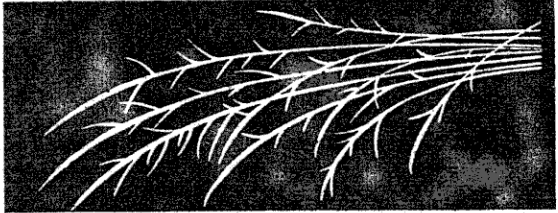
\includegraphics[width=0.7\linewidth]{Figuras/Ac_al_C.png}
    \caption{Acero al carbono dulce con 0,15\% de C.}
    \label{fig:0,15}
\end{figure}

\section{Características a Observar y Zonas de la Chispa.}

Para llevar a cabo el ensayo, se recomienda trabajar en un lugar con poca iluminación y utilizar una muela de grano y dureza media que gira alrededor de $1 500\: RPM$. Una chispa se divide en tres zonas principales:

\begin{enumerate}
    \item La más cercana a la muela, compuesta por rayos rectilíneos con el color característico del acero.
    \item Zona intermedia donde los rayos se bifurcan y ya aparecen algunas explosiones.
    \item La zona final, donde ocurren la mayor parte de las explosiones.
\end{enumerate}

\begin{figure}[h]
    \centering
    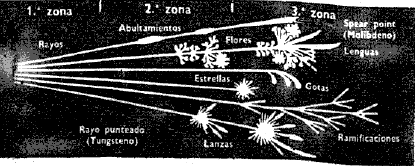
\includegraphics[width=0.7\linewidth]{Figuras/Zonas.png}
    \caption{Demarcación de zonas de las chispas.}
    \label{zonas}
\end{figure}

Las características clave para la identificación son la figura y el color. Se deben observar con detalle la longitud, el trazo (continuo, punteado, abultado) y la forma de las explosiones, que pueden ser estrellas, gotas, lenguas o flores.

\section{Clasificación por Elementos de Aleación.}

La forma y la intensidad de la chispa dependen de la composición del acero.
\begin{itemize}
    \item Aceros al Carbono: el grosor de los rayos, la luminosidad y la profusión de las explosiones aumentan a medida que se incrementa el porcentaje de carbono.
    \item Aceros con Molibdeno: Tienen una característica muy distintiva. En la extremidad de los rayos aparece una prolongación incandescente completamente separada, llamada \textacutedbl{}spear point\textacutedbl{}, de color rojo anaranjado.
    \item Aceros con Wolframio: Dan una chispa con rayos de color rojo oscuro, mucho menos luminosos que los de otras clases de aceros. En los aceros de alta velocidad (18\% de wolframio), los rayos son punteados y muy poco luminosos.
    \item Fundiciones: Las chispas de la fundición blanca, gris y maleable tienen características propias que permiten distinguirlas.
\end{itemize}

A continuación se presenta una tabla comparativa de lo dicho anteriormente:

\begin{table}[h!]
    \centering
    \begin{tabularx}{\textwidth}{>{\raggedright\arraybackslash}p{0.15\textwidth} >{\raggedright\arraybackslash}p{0.3\textwidth} >{\raggedright\arraybackslash}p{0.15\textwidth} >{\raggedright\arraybackslash}p{0.2\textwidth} >{\raggedright\arraybackslash}p{0.15\textwidth}}
        \toprule
        \textbf{Tipo de Material} & \textbf{Apariencia General de la Chispa} & \textbf{Rayos} & \textbf{Puntas
        /Explosiones} & \textbf{Elementos Clave} \\
        \midrule
        \textbf{Acero de Bajo Carbono} & Poco voluminosa, poco luminosa, poca longitud. & Rectilíneos, más largos. & Pocas explosiones, pequeñas. & - \\ \hline
        \textbf{Acero de Medio Carbono} & Más voluminosa y luminosa. & Más cortos. & Más explosiones, ramificadas. & Carbono \\ \hline
        \textbf{Acero de Alto Carbono} & Muy voluminosa y luminosa, muy ramificada. & Cortos y numerosos. & Muchas explosiones, con forma de hojas. & Carbono \\ \hline
        \textbf{Acero con Molibdeno} & Normal, pero con una característica distintiva. & Rectos. & Puntas de lanza (\textit{spear points}) al final de los rayos. & Molibdeno (Mo) \\ \hline
        \textbf{Acero Rápido (Wolframio)} & Muy corta, de volumen pequeño y color rojo oscuro. & Punteados, poco luminosos. & Ausencia casi total de explosiones. & Wolframio (W) \\ \hline
        \textbf{Acero para Troqueles} & Muy corta, con un color rojizo claro. & Rayos rectos y gruesos. & Puntas de lanza y pocas explosiones. & Molibdeno (Mo), Cromo (Cr), Manganeso (Mn), Vanadio (V) \\ \hline
        \textbf{Fundición Blanca} & Muy corta. & Rectos. & Explosiones grandes y en forma de hojas. & - \\ \hline
        \textbf{Fundición Gris} & Poca longitud, poco volumen, color naranja vivo. & Rectos. & Abundantes explosiones con forma de hojas. & Alto contenido de grafito \\ \hline
        \textbf{Fundición Maleable} & Muy voluminosa y larga. & Largos y rectos. & Ramificaciones abundantes y muy largas. & - \\ 
        \bottomrule
    \end{tabularx}
\end{table}

En \autoref{fig:aceros_y_fundiciones} se puede apreciar esquemáticamente las chispas y las diferencias entre ellas.

\begin{figure}[h!]
    \centering
    \begin{subfigure}{0.45\textwidth}
        \centering
        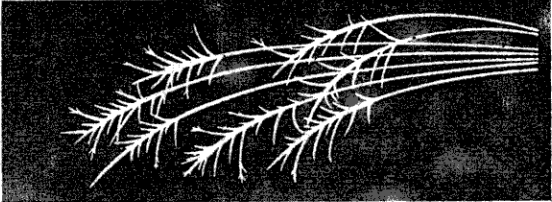
\includegraphics[width=\textwidth]{Figuras/0,32.png}
        \subcaption{Acero 0,32\% de C.}
        \label{fig:0,32}

        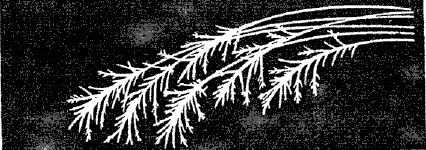
\includegraphics[width=\textwidth]{Figuras/0,42.png}
        \subcaption{Acero 0,42\% de C.}
        \label{fig:0,42}
    
        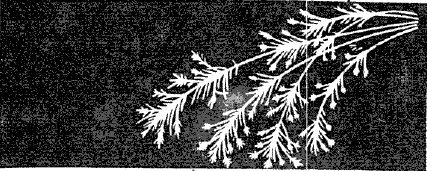
\includegraphics[width=\textwidth]{Figuras/1,05.png}
        \subcaption{Acero 1,05\% de C.}
        \label{fig:1,05}
    
        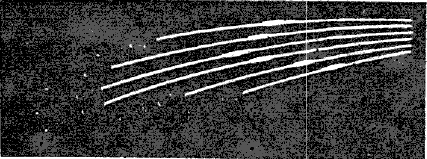
\includegraphics[width=\textwidth]{Figuras/Mo.png}
        \subcaption{Acero 0,32\% C; 0,5\% Mo.}
        \label{fig:Mo}
    \end{subfigure}
    \hfill
    \begin{subfigure}{0.45\textwidth}
        \centering
        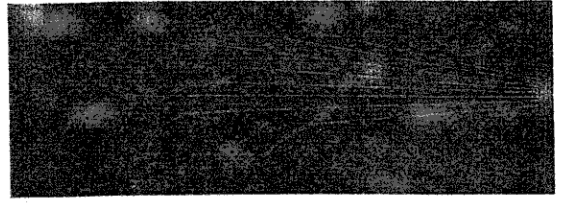
\includegraphics[width=\textwidth]{Figuras/W.png}
        \subcaption{Acero 18\% W.}
        \label{fig:W}
    
        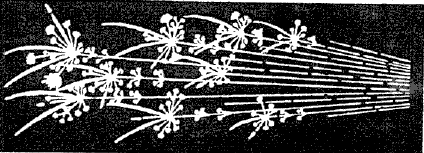
\includegraphics[width=\textwidth]{Figuras/troquel.png}
        \subcaption{Acero 2,2\% C; 12\% Cr.}
        \label{fig:troquel}
    
        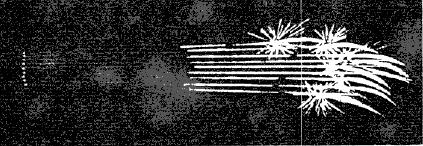
\includegraphics[width=\textwidth]{Figuras/blanca.png}
        \subcaption{Fundición blanca.}
        \label{fig:blanca}
    
        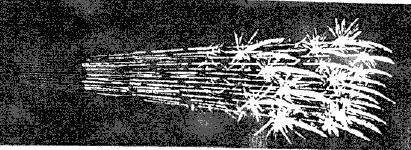
\includegraphics[width=\textwidth]{Figuras/gris.png}
        \subcaption{Fundición gris.}
        \label{fig:gris}
    \end{subfigure}
    \begin{subfigure}{0.8\textwidth}
        \centering
        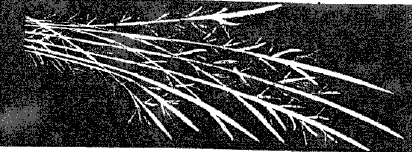
\includegraphics[width=\textwidth]{Figuras/maleable.png}
        \subcaption{Fundición maleable.}
        \label{fig:maleable}
    \end{subfigure}
    \caption{Distintas chispas de Aceros y Fundiciones.}
    \label{fig:aceros_y_fundiciones}
\end{figure}

\section{Limitaciones del Ensayo.}

El documento señala que el estado del material (templado o recocido) tiene poca influencia en la figura de la chispa, aunque puede afectar la facilidad con la que saltan y su brillo. Sin embargo, el estado superficial del material, como la cementación o la descarburación, puede falsear los resultados.


También, se destaca que el ensayo de chispa \textbf{no es útil para determinar la presencia de níquel} en los aceros, ya que este elemento no se manifiesta con ninguna característica particular en la chispa. Para el níquel, se debe recurrir a un ensayo químico complementario.

\vfill
\textit{\textbf{Este trabajo fue elaborado con la ayuda de la IA y otras páginas de ayuda para facilitar la confección y disposición de los elementos en dicho trabajo.}}

\end{document}